\documentclass{beamer}
\usetheme{Frankfurt} % http://deic.uab.es/~iblanes/beamer_gallery/
\usecolortheme{dove}
\setbeamertemplate{navigation symbols}{}
\makeatletter
\setbeamertemplate{footline}
{%
  \pgfuseshading{beamer@barshade}%
  \ifbeamer@sb@subsection%
    \vskip-9.75ex%
  \else%
    \vskip-7ex%
  \fi%
  \begin{beamercolorbox}[ignorebg,ht=2.25ex,dp=3.75ex]{section in head/foot}
    \insertnavigation{\paperwidth}
  \end{beamercolorbox}%
  \ifbeamer@sb@subsection%
    \begin{beamercolorbox}[ignorebg,ht=2.125ex,dp=1.125ex,%
      leftskip=.3cm,rightskip=.3cm plus1fil]{subsection in head/foot}
      \usebeamerfont{subsection in head/foot}\insertsubsectionhead
    \end{beamercolorbox}%
  \fi%
}%
\setbeamertemplate{headline}{}
\makeatother

\usepackage[T1]{fontenc}
\usepackage[utf8]{inputenc}
\usepackage[ngerman]{babel}
\usepackage[autostyle = true, german = quotes]{csquotes} % Anführungszeichen

\usepackage{amsmath}
\usepackage{graphicx}
\usepackage{epstopdf}

\begin{document}

%\subject{Praktikum Multicore"=Programmierung}
\title{Projekt~6: Mehrgittermethoden}
\author{Florian Klemme \and Manuel Leßmann}
\date{17.~Februar 2016}

\begin{frame}
    \titlepage
\end{frame}

\section*{Agenda}
\begin{frame}
    \tableofcontents
    \frametitle{Agenda}
\end{frame}

\section{Jakobi- und Gauß-Seidel-Verfahren}
\begin{frame}
    \frametitle{Jakobi und Gauß-Seidel}
    \begin{block}{Jakobi}
        \(u_{i,j}^{k} = (u_{i,j-1}^{k-1} + u_{i-1,j}^{k-1}
                       + u_{i,j+1}^{k-1} + u_{i+1,j}^{k-1}
                       + h^2 \cdot f(i \cdot h, j \cdot h)) \cdot 0.25;\)
    \end{block}
    \begin{block}{Gauß-Seidel}
        \(u_{i,j}^{k} = (u_{i,j-1}^{k} + u_{i-1,j}^{k}
                       + u_{i,j+1}^{k-1} + u_{i+1,j}^{k-1}
                       + h^2 \cdot f(i \cdot h, j \cdot h)) \cdot 0.25;\)
    \end{block}
    \centering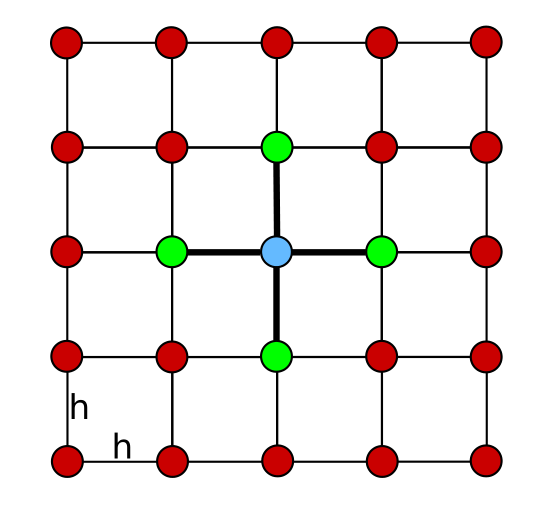
\includegraphics[width=0.4\textwidth]{jakobi-grid}
\end{frame}

\begin{frame}
    \frametitle{Jakobi und Gauß-Seidel}
    \begin{block}{Abbruchbedingungen}
        \begin{itemize}
            \item Maximale Anzahl an Iterationen
            \item Maximale Änderung zwischen zwei Iterationen unterschreitet Grenzwert
        \end{itemize}
    \end{block}
    \begin{block}{Qualitätsmetriken}
        \begin{itemize}
            \item Maximaler Fehler zur analytischen Lösung
            \item Mittlerer Fehler zur analytischen Lösung
        \end{itemize}
    \end{block}
\end{frame}

\subsection{Konvergenz}
\begin{frame}
    \frametitle{Konvergenz der Verfahren}
    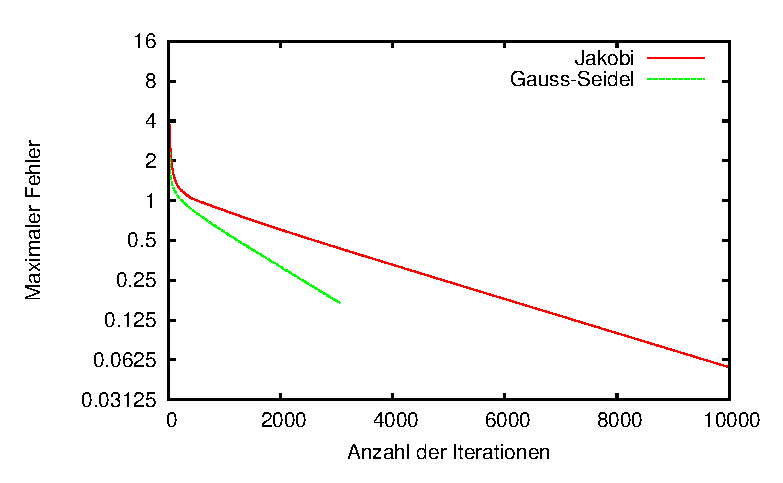
\includegraphics[width=\textwidth]{fehlerpresentation}
\end{frame}

\subsection{Parallelisierung mit OpenMP}
\begin{frame}
    \frametitle{Parallelisierung Jakobi}
    Trivial parallelisierbar:
    \begin{itemize}
        \item Keine Datenabhängigkeiten innerhalb einer Iteration
        \item Reduktion der Abbruchbedingung
        \item Statische Lastverteilung, da jedes Arbeitspaket gleich groß ist
        \item Ping-Pong-Verfahren zum effizienten Zugriff auf die vorherige Iteration
    \end{itemize}
    Aber:
    \begin{itemize}
        \item Hoher Overhead, da eine einzelne Iteration v.a. bei groben Gittern nicht sehr lange dauert
    \end{itemize}
\end{frame}

\begin{frame}
    \frametitle{Parallelisierung Gauß-Seidel}
    Datenabhängigkeiten innerhalb einer Iteration!
    \begin{itemize}
        \item Neuer Wert abhängig von den Werten links und oberhalb aus der aktuellen Iteration
    \end{itemize}
    Also: keine triviale Methode möglich.
\end{frame}

\begin{frame}
    \frametitle{Ansatz: Wavefront-Muster}
    \centering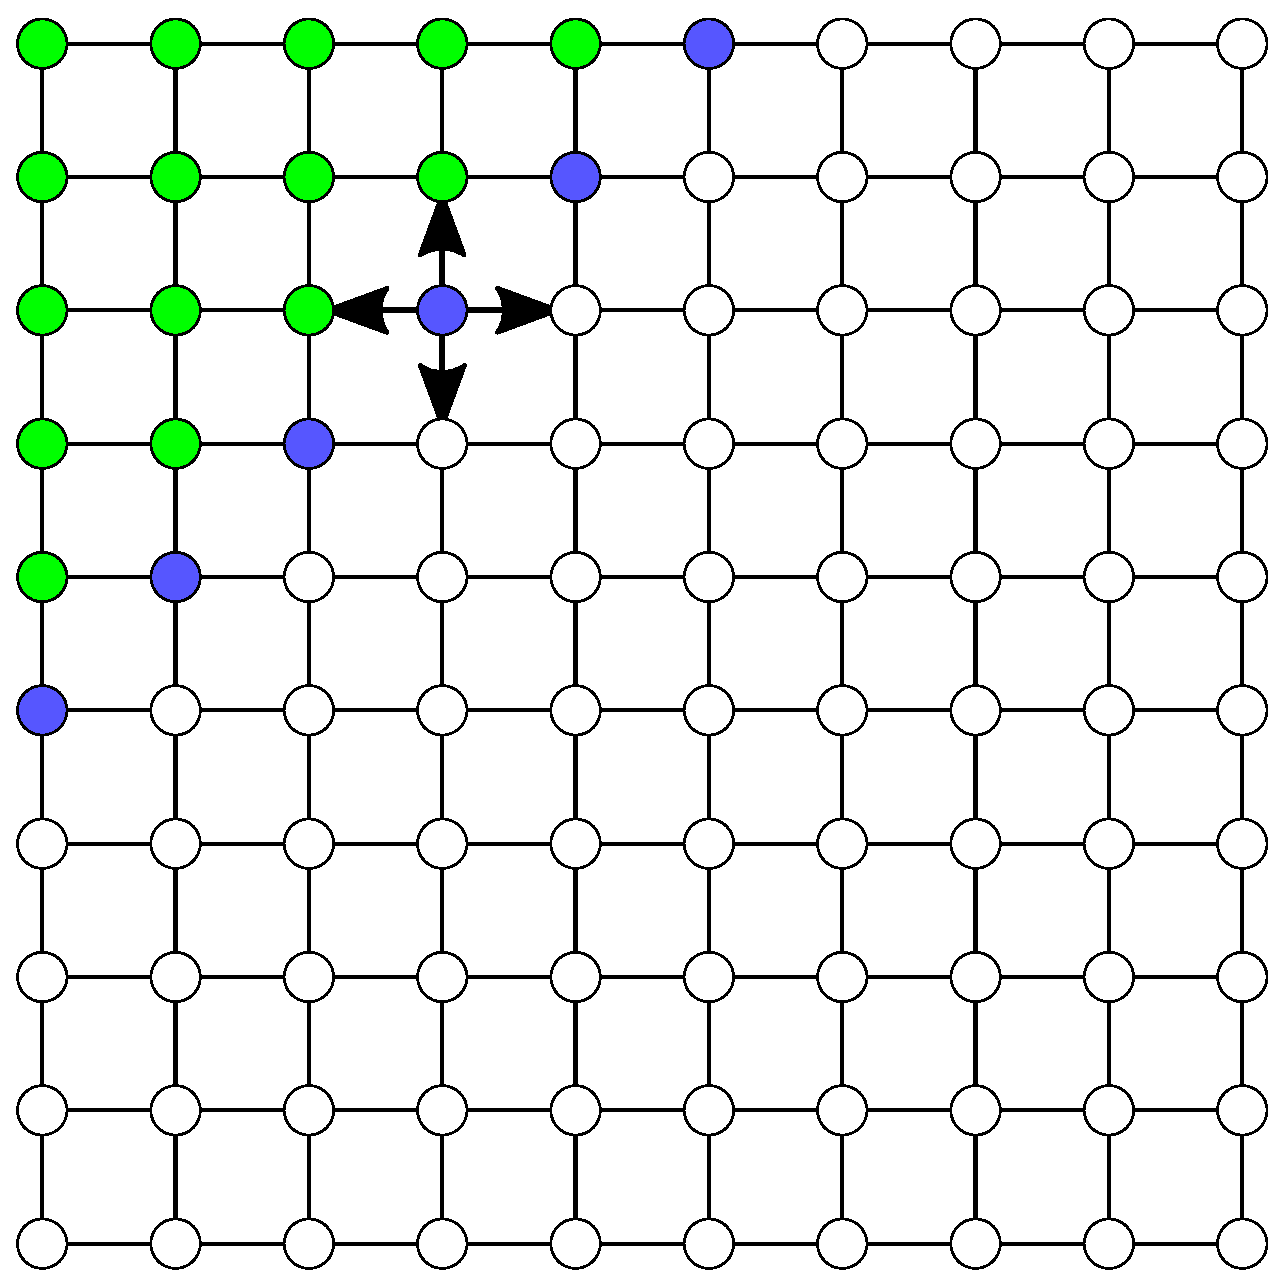
\includegraphics[width=0.5\textwidth]{wavefront-datadependencies}
\end{frame}

\begin{frame}
    \frametitle{Ansatz: Wavefront-Muster}
    \begin{columns}
        \begin{column}{0.5\textwidth}
            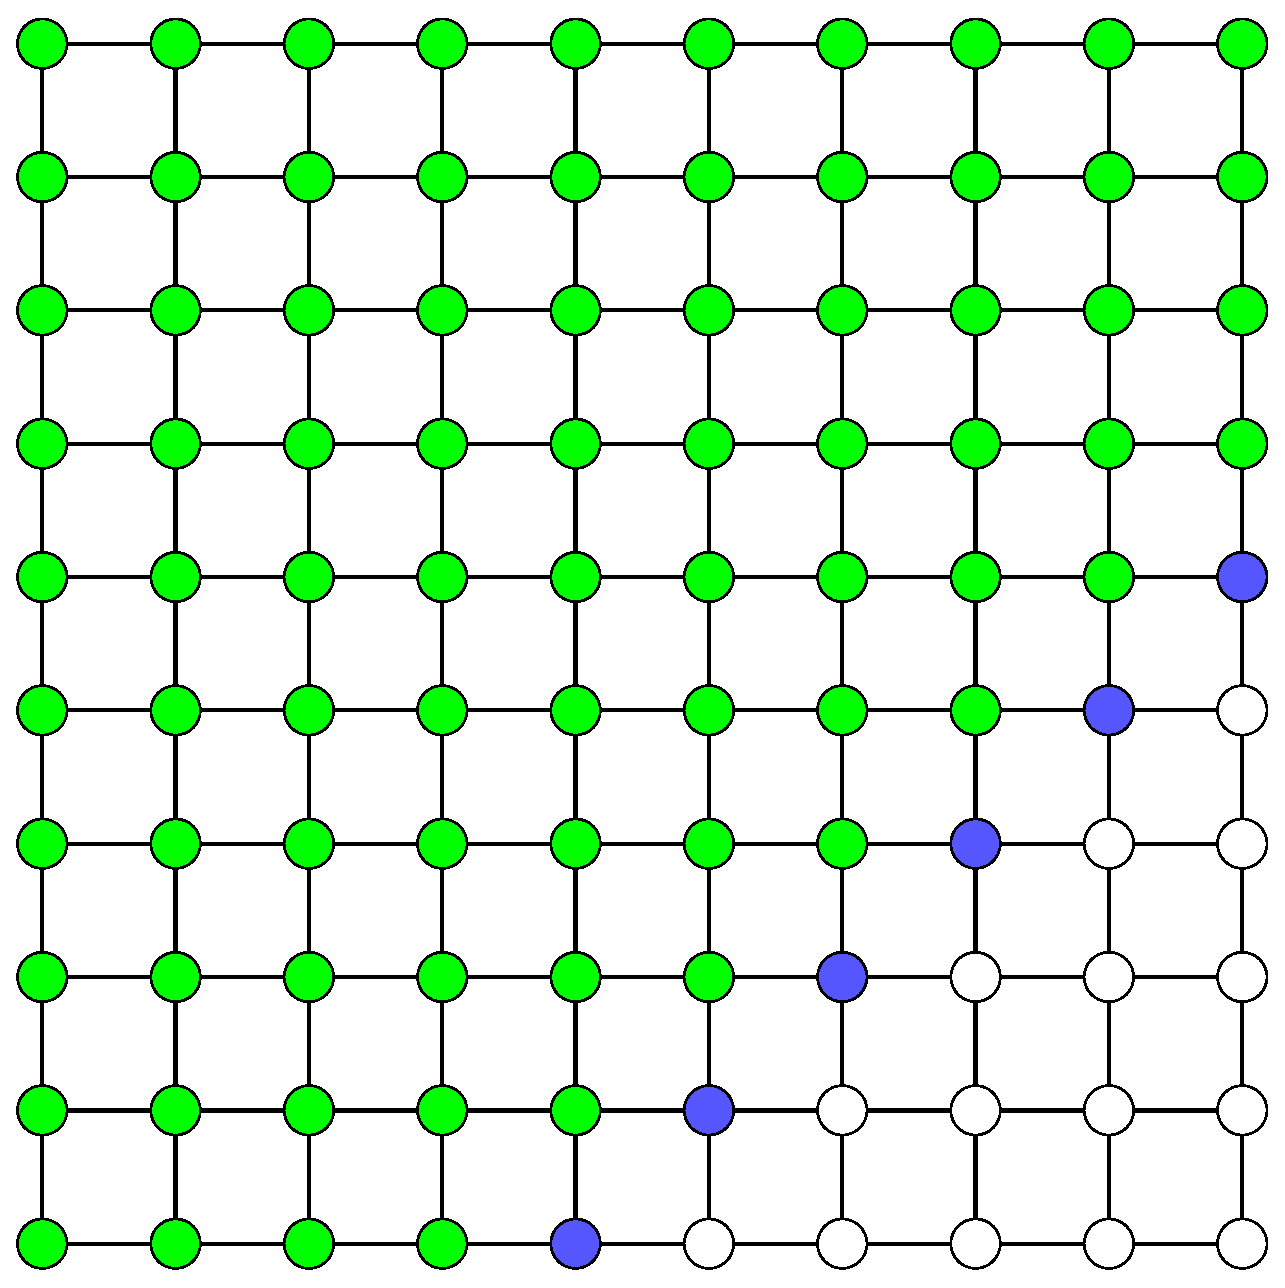
\includegraphics[width=\textwidth]{wavefront1}
                        
            \centering Iteration $n$
        \end{column}
        \begin{column}{0.5\textwidth}
            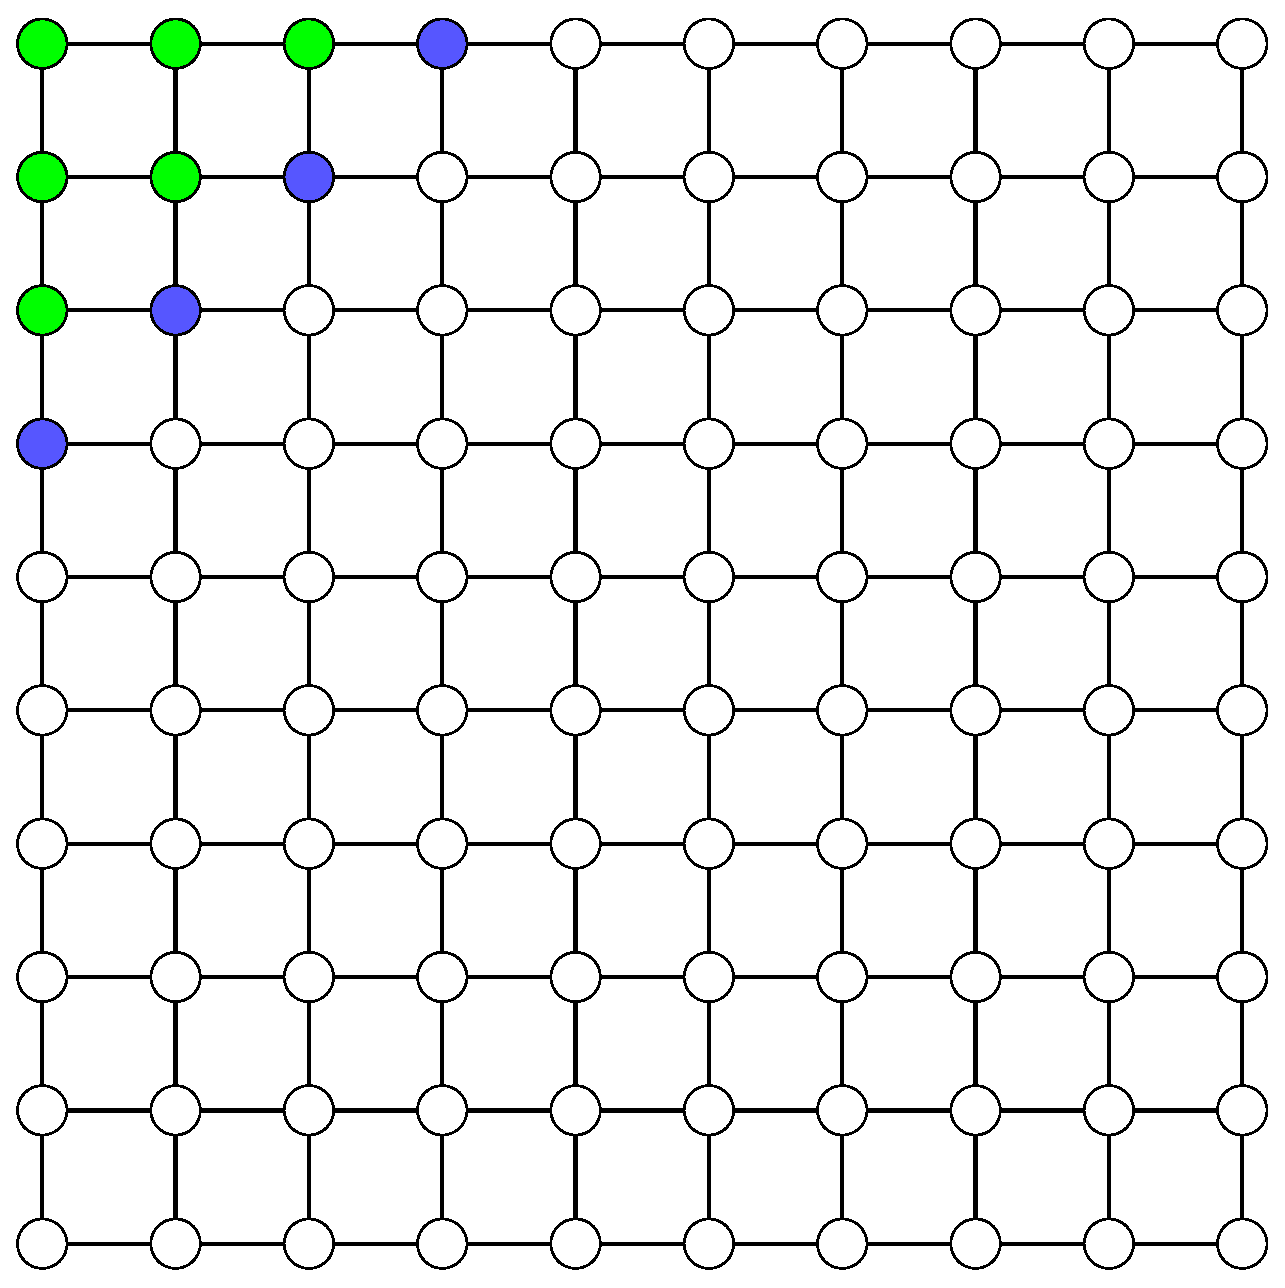
\includegraphics[width=\textwidth]{wavefront2}
            
            \centering Iteration $n+1$
        \end{column}
    \end{columns}
\end{frame}

\begin{frame}
    \frametitle{Parallelisierung Gauß-Seidel}
    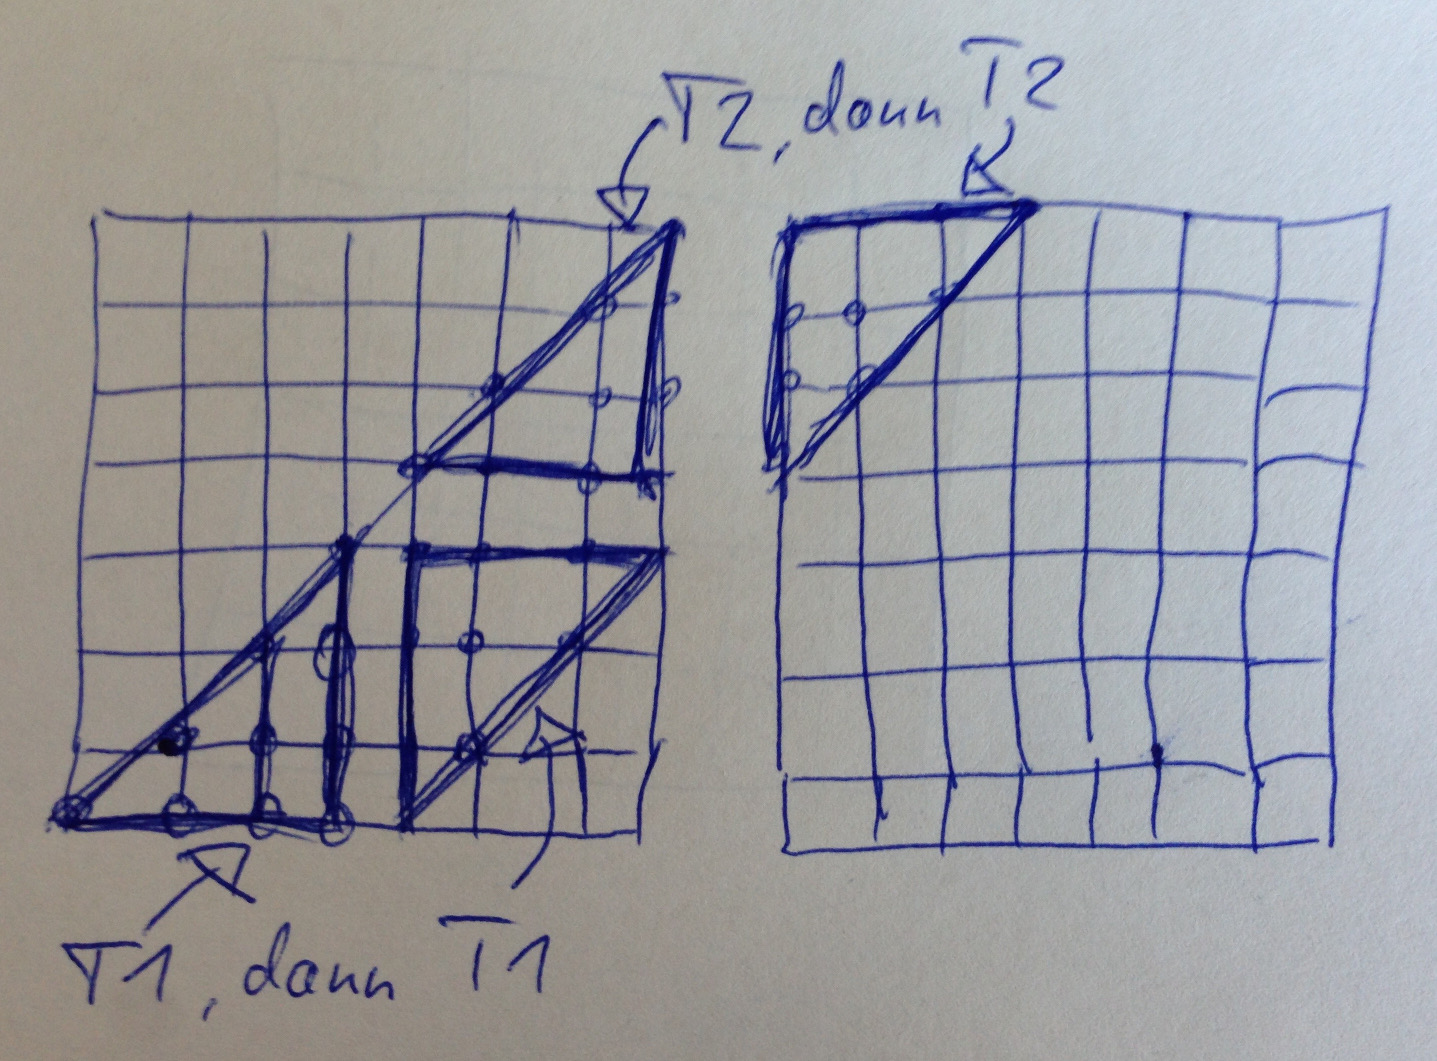
\includegraphics[width=\textwidth]{gaussseideldreiecke}
\end{frame}

\subsection{Speedup und Effizienz}
\begin{frame}
    \frametitle{Speedup und Effizienz: Jakobi Verfahren}
    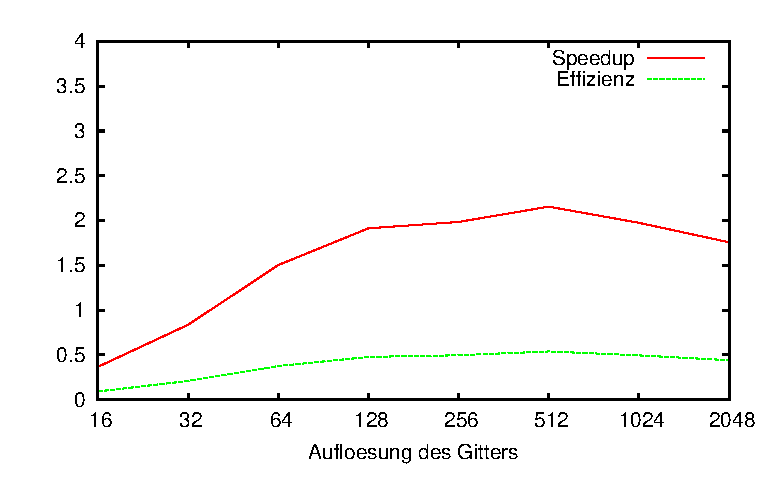
\includegraphics[width=\textwidth]{benchmarkjakobi}
\end{frame}

\begin{frame}
    \frametitle{Speedup und Effizienz: Gauß-Seidel Verfahren}
    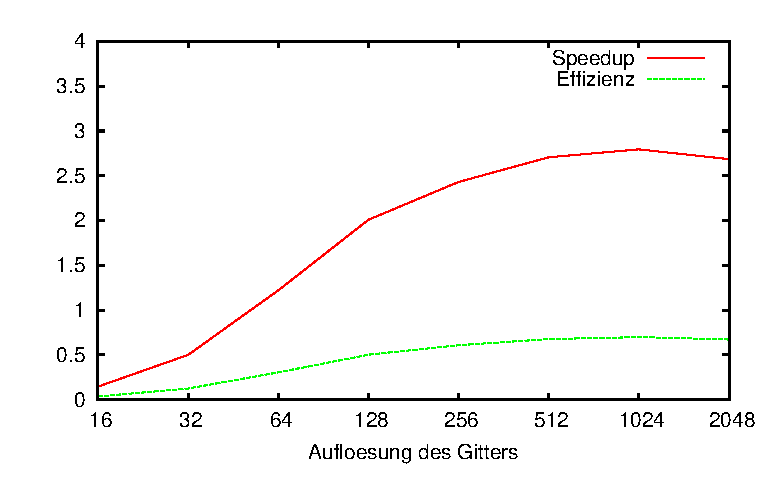
\includegraphics[width=\textwidth]{benchmarkgaussseidel}
\end{frame}

\section{Mehrgitter-Verfahren}
\begin{frame}
    \frametitle{Mehrgitter"=Verfahren}
    Hier erklären. Was ist das Problem / was ist die Idee?
\end{frame}

\subsection{Restriktion und Interpolation}
\begin{frame}
    \frametitle{Restriktion und Interpolation}
    Hier vielleicht das schicke Bild von der Vorlesung oder ähnliches.
\end{frame}

\subsection{Alpha"=Wert} % TODO: Besserer Titel?
\begin{frame}
    \frametitle{Alpha"=Wert}
    V"= und W"=Muster zeigen. Einfluss vom Alpha"=Wert erklären.
\end{frame}

\begin{frame}
    \frametitle{Fehlerverbesserung bei geringen \(z\)"=Werten}
    \begin{center}
    \begin{tabular}{|r|r|r|r|} \hline
    & & \multicolumn{2}{c|}{Approx. Fehler} \\
    n    & alpha & Mittel & Maximum \\ \hline \hline
    256  & 1     & 0,0771 & 0,1962  \\
    256  & 2     & 0,0771 & 0,1962  \\
    512  & 1     & 0,0431 & 0,1052  \\
    512  & 2     & 0,0431 & 0,1053  \\
    1024 & 1     & 0,0321 & 0,0853  \\
    1024 & 2     & 0,0222 & 0,0548  \\
    2048 & 1     & 0,2341 & 0,5783  \\
    2048 & 2     & 0,0111 & 0,0289  \\ \hline
    \end{tabular}
    \end{center}
    Konfiguration: \(z_1 = z_2 = 4, h_{max} = 16 \cdot h\)
\end{frame}

\subsection{Beispiel graphisch dargestellt}
\begin{frame}\frametitle{Beispielfunktion als Plot}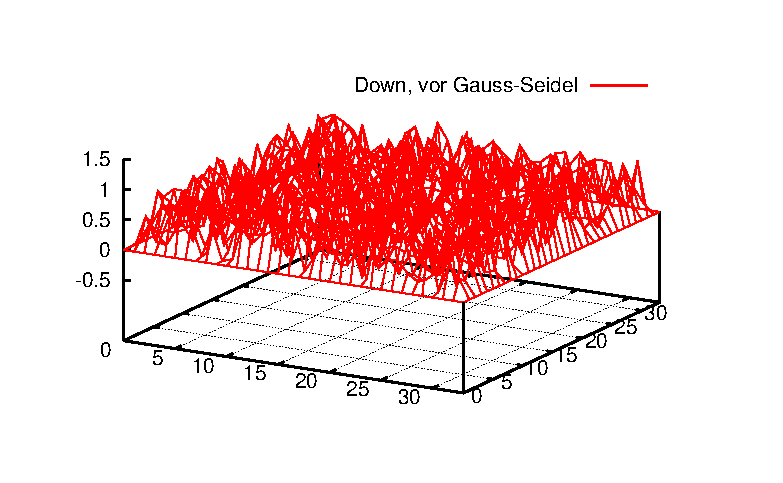
\includegraphics[width=\textwidth]{plots/000}\end{frame}
\begin{frame}\frametitle{Beispielfunktion als Plot}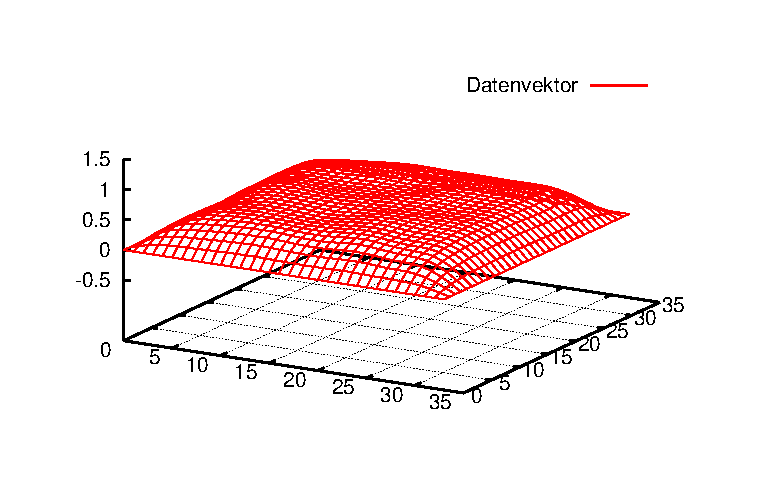
\includegraphics[width=\textwidth]{plots/001}\end{frame}
\begin{frame}\frametitle{Beispielfunktion als Plot}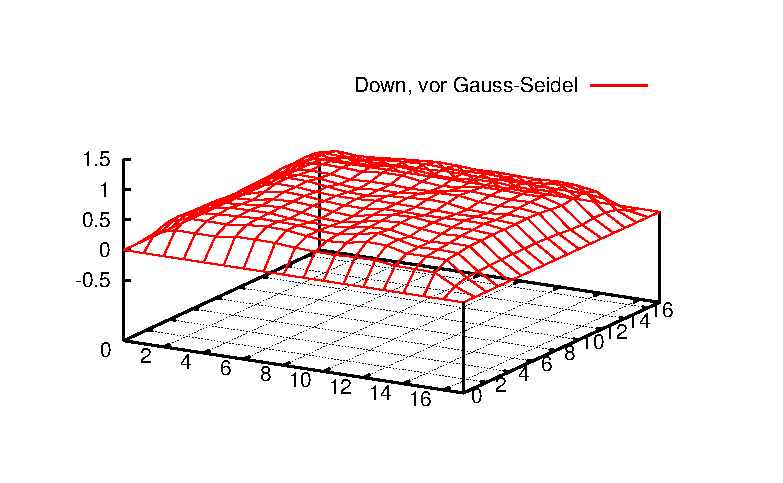
\includegraphics[width=\textwidth]{plots/002}\end{frame}
\begin{frame}\frametitle{Beispielfunktion als Plot}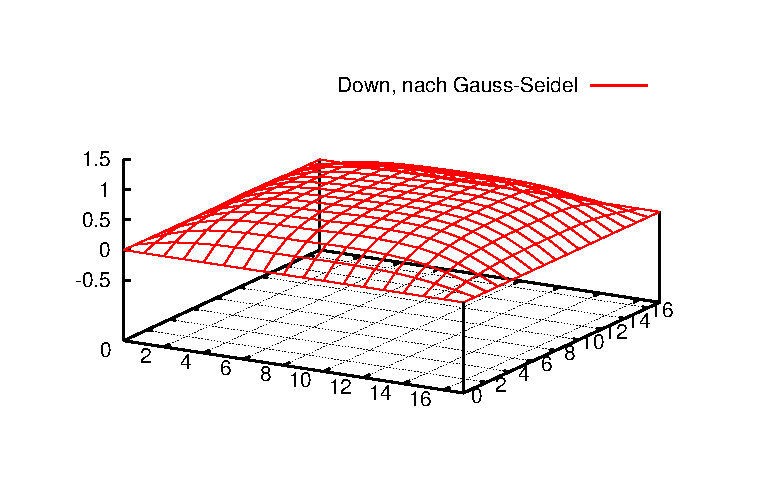
\includegraphics[width=\textwidth]{plots/003}\end{frame}
\begin{frame}\frametitle{Beispielfunktion als Plot}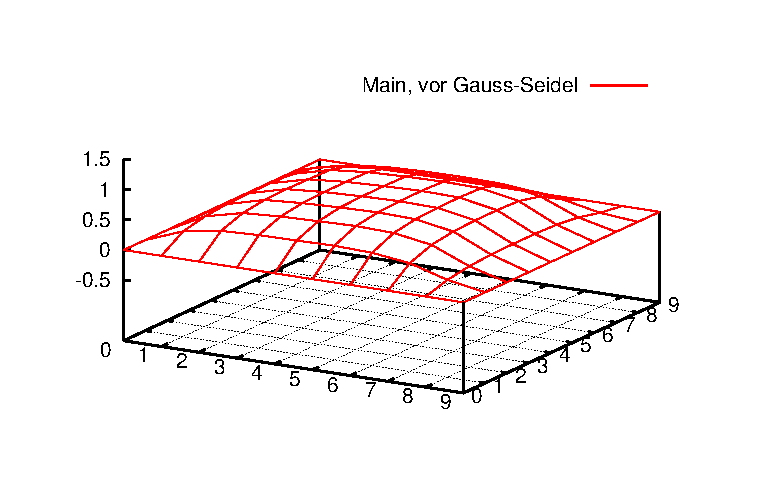
\includegraphics[width=\textwidth]{plots/004}\end{frame}
\begin{frame}\frametitle{Beispielfunktion als Plot}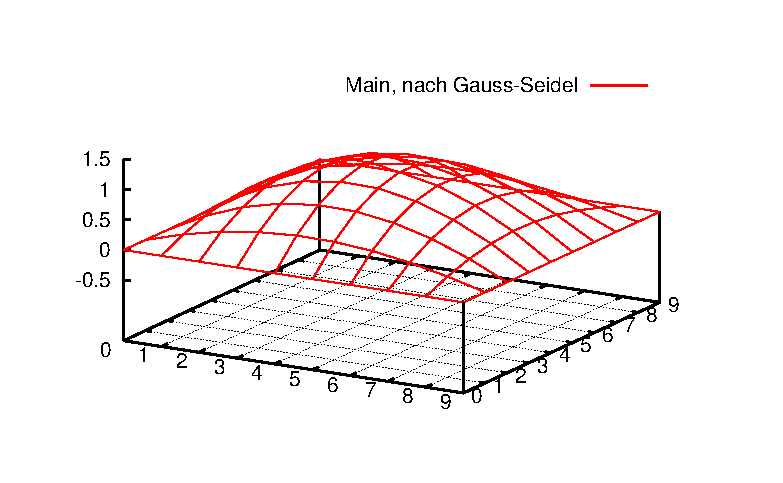
\includegraphics[width=\textwidth]{plots/005}\end{frame}
\begin{frame}\frametitle{Beispielfunktion als Plot}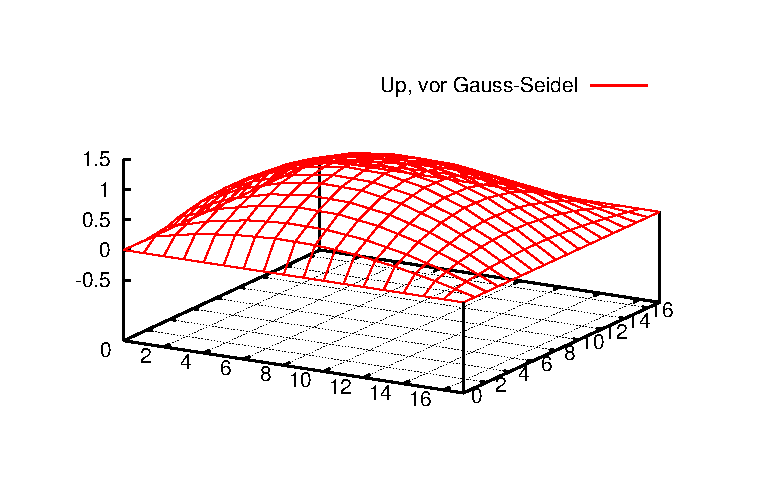
\includegraphics[width=\textwidth]{plots/006}\end{frame}
\begin{frame}\frametitle{Beispielfunktion als Plot}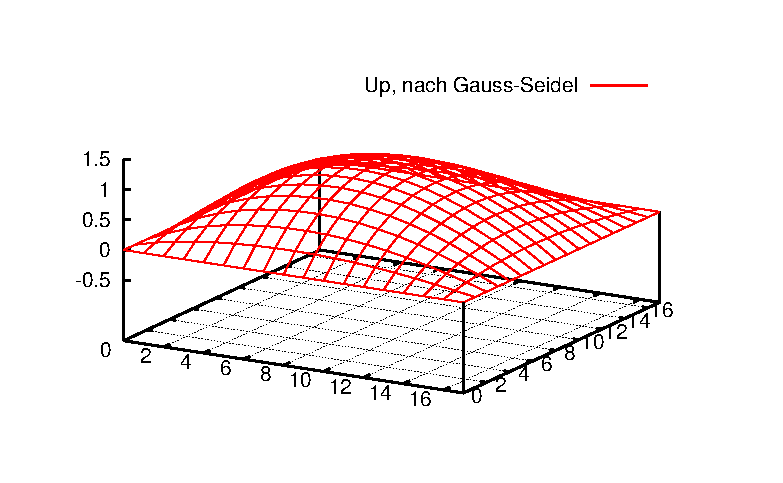
\includegraphics[width=\textwidth]{plots/007}\end{frame}
\begin{frame}\frametitle{Beispielfunktion als Plot}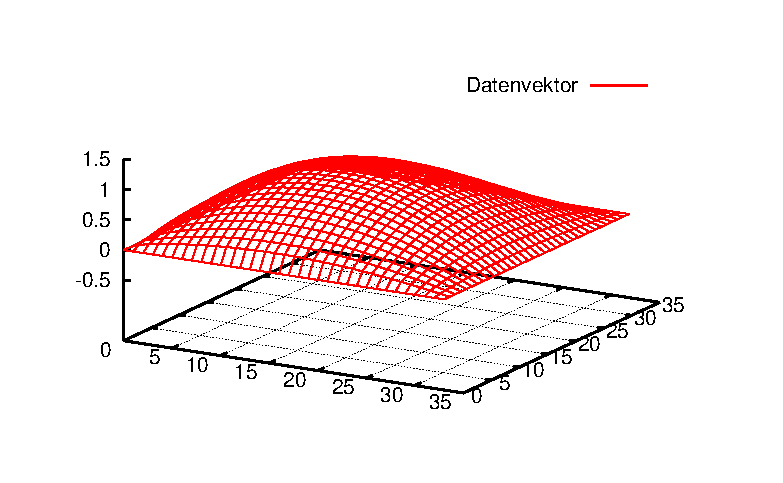
\includegraphics[width=\textwidth]{plots/008}\end{frame}
\begin{frame}\frametitle{Beispielfunktion als Plot}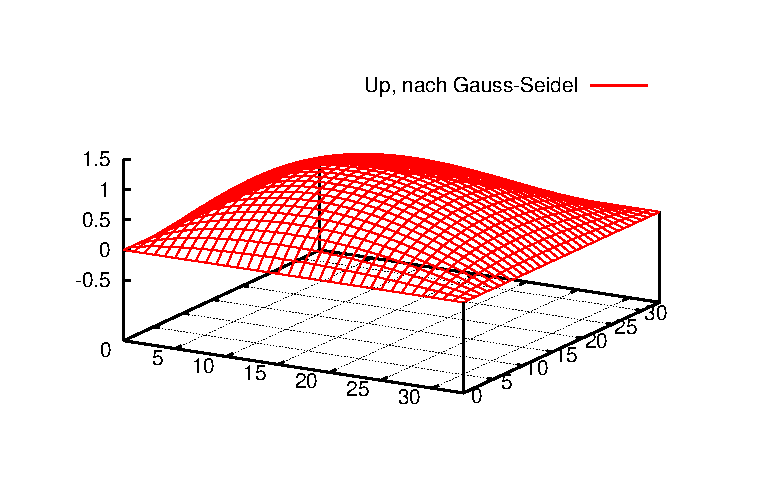
\includegraphics[width=\textwidth]{plots/009}\end{frame}

\subsection{Speedup und Effizienz}
\begin{frame}
    \frametitle{Skalierbarkeit des Mehrgitterverfahrens}
    \begin{center}
    \begin{tabular}{|r|r|r|r|r|} \hline
    & \multicolumn{2}{c|}{Laufzeit in Sekunden} & & \\
    n    & Sequentiell & Parallel & Speedup & Effizienz \\ \hline \hline
    16   & 0,0004      & 0,0072   & 0,0567  & 0,0142    \\
    32   & 0,0016      & 0,0139   & 0,1124  & 0,0281    \\
    64   & 0,0067      & 0,0379   & 0,1765  & 0,0441    \\
    128  & 0,0350      & 0,1045   & 0,3352  & 0,0838    \\
    256  & 0,1422      & 0,1522   & 0,9338  & 0,2334    \\
    512  & 0,5698      & 0,3205   & 1,7780  & 0,4445    \\
    1024 & 2,3061      & 0,9857   & 2,3397  & 0,5849    \\
    2048 & 9,2382      & 3,6254   & 2,5482  & 0,6371    \\ \hline
    \end{tabular}
    \end{center}
\end{frame}

\begin{frame}
    \frametitle{Laufzeiten im Vergleich}
    \footnotesize
    \begin{tabular}{|l|r|r|r|r|r|r|} \hline
    & \multicolumn{2}{c|}{Laufzeit in Sek.} & & & \multicolumn{2}{c|}{Approx. Fehler} \\
    Algorithmus & Seq.    & Parallel & Speedup & Effizienz & Mittel   & Maximum \\ \hline \hline
    Jakobi      & 33,9062 & 19,2902  & 1,7577  & 0,4394    & 0,4443   & 0,9990  \\
    Gauß-Seidel & 52,3843 & 19,5082  & 2,6853  & 0,6713    & 0,4436   & 0,9981  \\
    Mehrgitter  & 2,5800  & 1,3330   & 1,9354  & 0,4838    & 0,0111   & 0,0289  \\ \hline
    \end{tabular}
\end{frame}

\end{document}
